\documentclass{article}
\usepackage[utf8]{inputenc}
\usepackage{amsmath}
\usepackage{laskaripohja}
\usepackage{enumitem}
\usepackage{graphicx}
\usepackage{float}



% For python code. Use \begin{lstlisting}
\usepackage{listings}
\usepackage{xcolor}
\lstset{
    language=Python,
    basicstyle=\ttfamily\small,
    keywordstyle=\color{blue},
    commentstyle=\color{green!50!black},
    stringstyle=\color{red},
    showstringspaces=false,
    breaklines=true,
    frame=single
}




% Jos haluat kirjoittaa matikkaa nii dollarikirjain

\title{ML Project Stage 2 Report - Classifying near-earth objects using machine learning methods}
\author{}
\date{}

\begin{document}
\maketitle


\vspace{-1.9cm}

\section{Introduction}

A rare but ever-existing threat to our planet have been potentially hazardous NEO (near-earth objects). Around 40 thousand NEO are currently orbiting Earth \cite{neo_stats}. Most of the objects pose no threat and will either miss completely or burn up in the atmosphere. Still, being able to identify the ones that are potentially hazardous is crucial for our safety. Classifying the orbit of 40 thousand objects would be a horrifying task to do by hand. Given enough data, this could be something that computers can handle more efficiently. Our task is to explore machine learning methods that could reliably classify the NEO and speed up the process.


\vspace{1em}

Section 2 explains the problem formulation for this project as well as describes the labels for the data. Section 3 explains the preparation of the data for the task as well as the selection of models. Sections 4 and 5 present and discuss the results and conclusions. Section 6 explains the use of AI in this project, lastly are the references and code appendix listed.

\section{Problem formulation}


The objective for this project is to use machine learning to make a binary prediction: if a given NEO is potentially hazardous to earth or not. For this task we will use the ''NASA - Nearest Earth Objects'' dataset, found on Kaggle \cite{Kaggle_neo_data}. The dataset contains two files, ''neo.csv'' and ''neo\_v2.csv''. We will use the latter, as it is the updated and newer version. This is a supervised machine learning project because each object in the dataset is labeled as potentially hazardous or not.

\vspace{1em}

The data contains 10 different features, which are the following: ID, name, estimated minimum diameter, estimated maximum diameter, relative velocity, miss distance, orbiting body, sentry object, absolute magnitude, and hazardous. ID is a unique identifier for each asteroid, and names are given by NASA. The estimated minimum and maximum diameter is in kilometers. Relative velocity is in kilometers per hour and measured relative to earth. Miss distance is the closest distance that the object will come to earth during the particular orbit that the object was observed. Orbiting body is earth for all objects. Sentry object is a Boolean value of if the object is included in ''Sentry - automated collision monitoring system'', and is ''false'' for all objects. Absolute magnitude is a measure of the luminosity of an object. It is the negatively logarithmic ratio between the light flux from the object and a reference amount of light flux at the distance of one astronomical unit. A higher absolute magnitude ratio corresponds to a fainter object. It is a standardized measurement used in astronomical research. Hazardous is a Boolean value of if the object is a potentially hazardous object or not. This is the feature we are interested in predicting. 

%The data contains around 90 thousand rows of data of which around 27 thousand have a unique ID, thus several objects have been recorded more than once at different points of their orbits.

\vspace{1em}

The dataset contains discrete recordings of NEOs and their relevant traits. The data originates from NASA's NEO Earth Close Approaches database and was compiled by Sameep Vani, who is the owner of the dataset \cite{Kaggle_neo_data}.










\section{Methods}
\subsection{Preparing the data}


The dataset consists of 90,836 rows of data points. During the preliminary analysis, none of the entries were found to contain missing values, thus, none of the rows had to be removed or adjusted. The labels sentry\_object and orbiting\_body contained the same value for all objects and were therefore removed. Similarly, ID and name columns were removed since they did not provide any useful information for predicting if an object was potentially hazardous. Finally, the Boolean ''hazardous'' label was converted into binary values, where 1 represents a potentially hazardous object and 0 a non-hazardous object. The remaining labels were est\_diameter\_min, est\_diameter\_max, relative\_velocity, miss\_distance, absolute\_magnitude, hazardous, and hazardous\_int.




\vspace{1em}


%An examination of the ratios between hazardous and non-hazardous objects as well as correlation was performed to better understand the composition of the dataset. Out of the 90,836 data points 81,996 (90.27\%) were labeled as non-hazardous and 8,840 (9.73\%) were labeled as hazardous. The dataset is heavily skewed towards non-hazardous objects, and therefore accuracy alone would not be a reliable evaluation metric. If the model simply always guessed non hazardous it would reach an accuracy of around 90\% which could sound impressive, but would miss the inability of the model to detect any hazardous objects. Additional statistics such as standard deviation, mean, count, minimum and maximum values were calculated to visualize the data.

Out of the 90,836 data points, 81,996 (90.27\%) were labeled as non-hazardous, and 8,840 (9.73\%) were labeled as hazardous. The dataset is heavily skewed towards non-hazardous objects, and therefore accuracy alone would not be a reliable evaluation metric. %Additional statistics such as standard deviation, mean, count, minimum and maximum values were calculated to understand the dataset.


\iffalse
\begin{figure}[H]
    \centering
    \includegraphics[width=0.75\linewidth]{Screenshot 2026-09-18 at 14.06.07.png}
    \caption{Statistical measures of the dataset}
\end{figure}
\fi


\vspace{1em}


Pearson correlation was used to estimate the correlation between each feature and the hazardous integer feature. Absolute magnitude showed the strongest (negative) correlation of $r=-0.365$, followed by relative velocity at $r=0.191$. Intuitively this makes sense, as a larger object has more surface area to reflect light and therefore have a lower absolute magnitude. Both higher velocity and larger size make sense to be treated as a bigger threat. Estimated minimum and maximum diameter had a correlation of $r=0.183$. Miss distance had a correlation of $r=0.042$. Correlation between minimum and maximum diameter was found to be $r=1.0$. Since the min and max diameter had essentially identical correlations, only one of the features will be included going forward for the sake of reducing redundancy. The maximum estimated diameter was chosen to be kept, as it provides an upper limit to the size of an object that could be potentially hazardous. %Miss distance was included as a feature as it is a relevant factor in how close an object comes to earth.


\vspace{1em}


The data was split into training, validation, and test ratio of 64/16/20 using the train\_test\_split function twice. We used stratification to approximately preserve the ratios in each dataset and saved them in separate files. The training, validation and test datasets contained 52,476/5,658, 13,120/1,414, and 16,400/1,768 non-hazardous/hazardous data points each, respectively. These ratios are nearly identical and will work well for this project.

\iffalse
\vspace{1em}

Underneath is a visualisation of the distribution of non-hazardous-to-hazardous and a distribution of the size of the objects. The horizontal axis for the size is scaled logarithmically, as most of the objects are of smaller size.


\begin{figure}[H]
    \centering
    \includegraphics[width=0.9\linewidth]{visualisation.png}
    \caption{Visualisation of the dataset}
\end{figure}
\fi

\subsection{Models}

The first method chosen for this project is logistic regression, since it is a relatively simple model that is designed to produce a binary output. Logistic regression creates a linear function with weights based on the training data and runs the linear function through the sigmoid function to classify the input. Because the data is heavily skewed towards non-hazardous objects, we will set the class\_weight parameter to balanced to help the model better pick out potentially hazardous objects. Scikit-learn’s logistic regression uses the logarithmic loss function to adjust its weights. %\cite{logisticregression}.

%The choice of method for this project is logistic regression, since it is a relatively simple and intuitive regression model that is designed to produce a binary output, and handles numerical input values well. Logistic regression creates a linear function with weights based on the training data and runs the linear function through the sigmoid function to classify the input \cite{logisticregressoion}.


\vspace{1em}

The hypothesis space is the set of all possible logistic regression functions defined as below, where $x$ is the vector of recorded feature values for an object, $\mathbf{w}$ is the vector containing the weights, b is the bias term, and $\sigma$ is the sigmoid function.

\begin{align*}
    \mathcal{H} = \{\sigma(\mathbf{w}^Tx + b) \ | \ \mathbf{w}\in \mathbb{R}^4, b\in\mathbb{R} \} \ , \ \ \sigma(z) = \frac{1}{1+e^{-z}}
\end{align*}



The logarithmic loss function is defined below, where $y$ is the true value and $p$ is the predicted value. % \cite{logloss}.

\begin{align*}
    L_{log}(y,p) = -\left(y \log (p) + (1-y) \log (1-p)\right)
\end{align*}



The second method chosen for this task was gradient boosting. Gradient boosting trains multiple regression trees sequentially, where each new tree is trained in a way that minimizes the loss of the current combined model. Scikit-learn’s gradient boosting model uses the same logarithmic loss function as logistic regression. Regression trees tend to perform decently in binary classification, and gradient boosting handles nonlinearities even better than typical regression trees. Because the features did not show a notably high correlations with the hazardous feature, we suspected there may exist nonlinear relationships, which is why we chose to use gradient boosting model to handle these potential nonlinearities.


\vspace{1em}

The hypothesis space for gradient boosting is the set of all functions constructed by additive combination of decision trees. After tuning the model, we got the best results by having n\_estimators=200, learning\_rate=0.2 and max\_depth=5.

%We will use the default hyperparameters for our model, except random state being set to 42 to get consistent results, which means that the model will consist of 200 regression with each having a maximum depth of 5.






% The miss distance is the closest an object will come during a particular orbit that it was, not the overall closest it will ever be to earth. That would be an incredibly difficult task to measure because of the amount of objects of different sizes that could slightly alter the orbit and have a butterfly effect and suddenly hit earth.


\section{Results}

Because of the data being heavily skewed towards non-hazardous NEO, we used three different metrics to determine the effectiveness of the model, accuracy, recall, and precision. Accuracy measures the proportion of correctly categorized objects, recall measures the proportion of potentially hazardous NEO it detects, and precision measures how often the model was right when it guessed ''hazardous''. %Because of our previous split, we did not include validation error and simply used training and test errors.

\vspace{1em}

% RESULTS!!
Logistic regression had a training error of 0.218 and a validation error of 0.216, and on the validation set it got an accuracy of 0.782, a recall of 0.930 and a precision of 0.300. Gradient boosting had a training error of 0.060 and a validation error of 0.084, and on the validation set it got an accuracy of 0.916, a recall of 0.264, and a precision of 0.671.

\vspace{1em}

Despite gradient boosting having a higher accuracy, its lower recall of 0.264 suggests that it was not able to detect a significant portion of the potentially hazardous NEO. The validation error being around 40\% higher than the test error for gradient boost suggests it was potentially overfitting. On the other hand, logistic regression having a precision of 0.300 suggests that only a third of the objects labeled as potentially hazardous were actually potentially hazardous. While tuning the models, we noticed that a small increase in recall for gradient boosting brought the precision significantly down, and similarly a small increase in precision brought the recall significantly down for logistic regression. In the case of potentially hazardous NEO, it is better to be falsely alarmed than miss a potential hazard, which is why logistic regression was chosen as our final model.



\vspace{1em}

During the data processing stage the data was split into three datasets of ratios 64/16/20 using stratification to preserve the ratios of hazardous and non-hazardous in all datasets, and each dataset was saved in a separate .csv file. The test dataset had 16,400/1,768 non-hazardous/hazardous objects.

%The file containing only training data was used for training, and neither model had had access to the file containing test data before this point.

\vspace{1em}

Since this is a binary classification task, we used 0-1 loss to calculate the test error. The test error for our final logistic regression model was found to be 0.214. The model had an accuracy of 0.786, recall of 0.934, and precision of 0.304. These results suggest the model is able to pick out potentially hazardous objects at a high rate, but around 70\% of the objects classified as potentially hazardous are false positives. The test error is nearly identical to the validation- and training error, which does not suggest the model was over- or underfitting. Below is a confusion matrix of the results.

\begin{figure}[H]
    \centering
    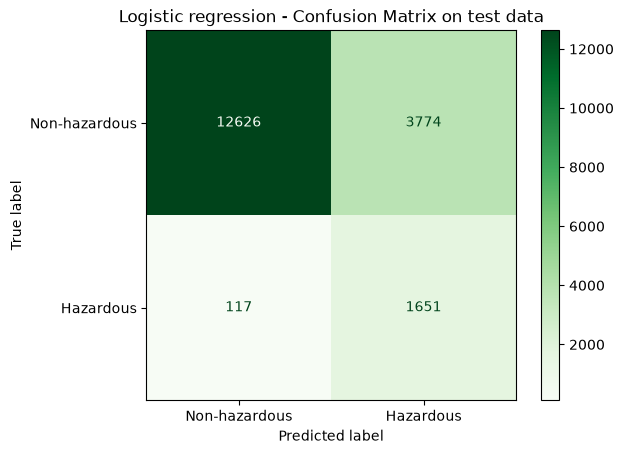
\includegraphics[width=0.48\linewidth]{finalconfusionmatriglogisticregression.png}
    \caption{Confusion matrix for logistic regression on test data}
\end{figure}



%DISCUSSION AND FINAL CHOSEN METHOD or apparently this is in conclusion part






\iffalse
\begin{figure}[H]
    \centering
    \includegraphics[width=0.75\linewidth]{ml_project_confusion_matrix.png}
    \caption{Confusion matrices for each model}
\end{figure}
\fi


\section{Conclusion}


This project aimed to find a machine learning method that would reliably detect near-earth objects that were potentially hazardous. The dataset used for this project contained measurements by the NASA NEO Earth Close Approaches database. The methods chosen for this project were logistic regression and gradient boosting. For each method, the error, accuracy, recall, and precision were calculated to determine their effectiveness.


\vspace{1em}

The results showed that neither method provided an ideal solution for predicting if a NEO was potentially hazardous or not. Logistic regression was chosen as the final method to apply on the testing data, as it showed substantially higher ability to detect potentially hazardous objects, as reflected by its high recall. The downside was that the high detection rate meant it picked up a lot of false positives, as around 70\% of the objects classified as potentially hazardous were false positives. The performance of the logistic regression stayed the same in the validation and test data, which suggests it was relatively stable and generalized reasonably well to unseen data. Gradient boosting appeared initially promising as a potential model with a low error, but further results showed that it was not able to reliably detect the potentially hazardous NEO.

\vspace{1em}


 These results demonstrate why simply looking at one metric, such as accuracy, is not always enough for determining how well a model works. In our case, as we saw a clear tradeoff between precision and recall, the desired model can depend a lot on the end user and their goals. This project prioritized recall while aiming to maintain an reasonable level of precision.

 \vspace{1em}

 The data being heavily skewed made classification more difficult and made accuracy a less useful measure, and there are several ways to make improvements in the future. The results suggest that a different machine learning model could potentially perform better than the two models we tested. In addition, finding data with more features could potentially help a machine learning model differentiate the NEO better.

 \vspace{1em}

In conclusion, neither logistic regression nor gradient boosting provided an ideal balance between detecting potentially hazardous NEO and limiting false positives. Logistic regression performed well in detecting potentially hazardous objects but suffered from having a significant amount of false positives, while gradient boosting had greater accuracy but significantly lower recall. To automate the task of classifying NEO, further models need to be tested, and data with more features may be considered.
 


% THEN HERE POTENTIAL REASONS FOR THOSE FINDINGS AND POTENTIAL IMPROVEMENTS
% ALSO HERE THAT IT'S NOT AS SIMPLE AS LOOKING AT ONE METRIC BUT DEPENDS ON WHAT THE END USER WANTS


% THEN IN CONCLUSION

%Despite tuning our models, we were not able to produce a model that would reliably detect the majority of the potentially hazardous objects while keeping the number of false positives low. A small increase in recall for gradient boosting brought precision significantly down, and similarly a small increase in precision brought recall significantly down for logistic regression. %This shows how difficult it can be to balance a model when the data is heavily skewed in one direction.

%\vspace{1em}


% THE RESULTS SHOWED.... you don't need to present them.

%Gradient boosting ended up having a higher accuracy of 0.916, which may seem promising at first, but was much worse at detecting the potentially hazardous NEO with a recall of 0.264.

%Logistic regression had a recall  of 0.930 but a precision of 0.300. Because being warned about a potential threat, even if false, is often more useful, we chose logistic regression as our final model

%\vspace{1em}

%these results suggest the task may require more data to better differentiate potentially hazardous from non hazardous or a more advanced machine learning model


%changing the threshold did unfortunately not bring significant improvements as the model quickly started to miss a significant amount of hazardous objects, but changing it to weight class balanced helped.

\section{Use of AI}


%\vspace{1em}

%Generative AI has been used in certain parts of this project. The usage has been limited to the following elements.


During the first week of this project, generative AI (Claude and ChatGPT) was used to brainstorm potential ideas that fit the scope of the project for this course, but generative AI has not been used in the choice of selecting the exact research question, problem formulation, or in choosing the dataset. Generative AI (Claude and ChatGPT) has also been used and limited to explaining library documentation for the libraries used in this project during the coding phase. All the code and structure of the code has been created by hand.



\bibliographystyle{IEEEtran}
\bibliography{sources.bib}



\section*{Appendices}


\begin{lstlisting}
""" Imports and loading the data"""
import pandas as pd
import numpy as np
import matplotlib.pyplot as plt
from sklearn.model_selection import train_test_split
from pathlib import Path

PROJECT_ROOT = Path.cwd().parent
csv_path = PROJECT_ROOT / "archive" / "neo_v2.csv"
df = pd.read_csv(csv_path)

print("Shape:", df.shape)
df.dtypes

print("Missing values per column:")
df.isnull().sum()   # Each cell 1 / 0 -> adds them together

\end{lstlisting}

\begin{lstlisting}
""" Change hazardous from (True/False) to (1/0)"""
df["hazardous_int"] = df["hazardous"].astype(int)
df = df.drop(columns=["hazardous"])  # (boolean) dropped, hazardous_int kept

print("Remaining columns:", list(df.columns))


""" Dropping non-informative columns """
print("Unique values in orbiting_body:", df["orbiting_body"].unique())  # Check for unique values
print("Unique values in sentry_object:", df["sentry_object"].unique())

drop_cols = ["id", "name"]
if df["orbiting_body"].nunique() == 1:  # Distinct value count, exclude Nan
    drop_cols.append("orbiting_body")
if df["sentry_object"].nunique() == 1:
    drop_cols.append("sentry_object")


df = df.drop(columns=drop_cols) # Removes columns from dataframe
print("Dropped columns:", drop_cols)
print("Remaining columns:", list(df.columns))

\end{lstlisting}


\begin{lstlisting}
""" Correlation """
numeric_cols_with_min =  ["est_diameter_min", "est_diameter_max",
                        "relative_velocity", "miss_distance", "absolute_magnitude"]

print("Correlation between est_diameter_min and est_diameter_max:",
      df["est_diameter_min"].corr(df["est_diameter_max"]))

print()
print("Correlation of each feature with the target:")
df[numeric_cols_with_min + ["hazardous_int"]].corr()["hazardous_int"]    # Pearsons correlation coefficient

\end{lstlisting}


\begin{lstlisting}
""" Drop est_diameter_min because of correlation with est_diameter_max"""
df = df.drop(columns=["est_diameter_min"])

numeric_cols = ["est_diameter_max", "relative_velocity", "miss_distance", "absolute_magnitude"]
print("Remaining columns:", list(df.columns))

\end{lstlisting}



\begin{lstlisting}
""" Summary of statistics"""
df[numeric_cols].describe()

""" Checking "ratio" between hazardous and non-hazardous"""
print(df["hazardous_int"].value_counts())  # Count how many times hazardous int appears
print()
print(df["hazardous_int"].value_counts(normalize=True) * 100)
\end{lstlisting}


\begin{lstlisting}
""" Visulaization """
fig, axes = plt.subplots(1, 2, figsize=(15, 4))

df["hazardous_int"].value_counts().plot(kind="bar", ax=axes[0])
axes[0].set_title("Class balance")
axes[0].set_xlabel("Hazardous")
axes[0].set_ylabel("Count")

axes[1].hist(np.log1p(df["est_diameter_max"]), bins=50)
axes[1].set_title("log(1 + est_diameter_max)")
axes[1].set_xlabel("log diameter (km)")

plt.tight_layout()
plt.show()


""" Save output, figures and data """
df.to_csv("clean_data.csv", index = False)
fig.savefig("plot_overview.png", dpi = 150)

print("Shape of clean_data.csv:", df.shape)
print("Columns in clean_data.csv", list(df.columns))
\end{lstlisting}


\begin{lstlisting}
""" Splitting clean_data.csv to train/test data"""
clean_df = pd.read_csv("clean_data.csv")

print("Shape", clean_df.shape)
print("Columns:", list(clean_df.columns))

train_val_data, test_data = train_test_split(
    clean_df,
    test_size = 0.2,
    stratify=clean_df["hazardous_int"], # Splits hazardous_int evenly
    random_state=42   # Same split each time you run the cell
)

train_data, validation_data = train_test_split(
    train_val_data,
    test_size=0.2,
    stratify=train_val_data["hazardous_int"],
    random_state=42
)

print("\n")
train_data.to_csv("train_data.csv", index=False)
print("train_data.csv saved")
validation_data.to_csv("validation_data.csv", index=False)
print("validation_data.csv saved")
test_data.to_csv("test_data.csv", index=False)
print("test_data.csv saved")
print("\n")

\end{lstlisting}


\begin{lstlisting}

print("Train data shape", train_data.shape)
print(train_data["hazardous_int"].value_counts())
print(train_data["hazardous_int"].value_counts(normalize=True) * 100)
print("\n")
print("Validation data shape:", validation_data.shape)
print(validation_data["hazardous_int"].value_counts())
print(validation_data["hazardous_int"].value_counts(normalize=True) * 100)

print("\n")
print("Test data shape", test_data.shape)
print(test_data["hazardous_int"].value_counts())
print(test_data["hazardous_int"].value_counts(normalize=True) * 100)

\end{lstlisting}

\begin{lstlisting}
""" Libraries needed for Stage 2 """

from sklearn.preprocessing import StandardScaler
from sklearn.linear_model import LogisticRegression
from sklearn.metrics import confusion_matrix, ConfusionMatrixDisplay
from sklearn.ensemble import GradientBoostingClassifier
from sklearn.metrics import accuracy_score

""" Load train / validation / test data and scaling it """

train_data = pd.read_csv("train_data.csv")
validation_data = pd.read_csv("validation_data.csv")
test_data = pd.read_csv("test_data.csv")

feature_cols = ["est_diameter_max", "relative_velocity", "miss_distance", "absolute_magnitude"]

X_train = train_data[feature_cols]
y_train = train_data["hazardous_int"]

X_validation = validation_data[feature_cols]
y_validation = validation_data["hazardous_int"]

X_test = test_data[feature_cols]
y_test = test_data["hazardous_int"]

scaler = StandardScaler()
X_train_scaled = scaler.fit_transform(X_train)
X_validation_scaled = scaler.transform(X_validation)
X_test_scaled = scaler.transform(X_test)
    # y data is boolean
\end{lstlisting}


\begin{lstlisting}
""" Logistic Regression"""

model = LogisticRegression(class_weight='balanced')
model.fit(X_train_scaled, y_train)  # Finding weights and Biases

print("Logisitc Regression fitted")
print("Weights: ", model.coef_)
print("Bias: ", model.intercept_)

""" Prediction on validation set """
y_pred = model.predict(X_validation_scaled)
y_pred_train = model.predict(X_train_scaled)


""" Confusion matrix of the Logisitc Regression """

cm = confusion_matrix(y_validation, y_pred)
print("Logisitc Regression Confusion matrix:")
print(cm)

# Visualization of the confusion matrix
disp = ConfusionMatrixDisplay(confusion_matrix=cm, display_labels=["Non-hazardous", "Hazardous"])
disp.plot(cmap="Greens") 
plt.title("Logistic Regression - Confusion Matrix")
plt.show()

\end{lstlisting}


\begin{lstlisting}
""" Validation confusion matrix analysis (Logisitic Regression) """

TN_LG = cm[0][0]
FP_LG = cm[0][1]
FN_LG = cm[1][0]
TP_LG = cm[1][1]

accuracy = (TP_LG + TN_LG) / (TP_LG + TN_LG + FP_LG + FN_LG)

if (TP_LG + FP_LG) > 0:
    precision = TP_LG / (TP_LG + FP_LG)
else:
    precision = 0

if (TP_LG + FN_LG) > 0:
    recall = TP_LG / (TP_LG + FN_LG)
else:
    recall = 0

if (precision + recall) > 0:
    f1 = 2 * (precision * recall) / (precision + recall)
else:
    f1 = 0

print("Validation metrics logistic regression")
print(f"Accuracy:  {accuracy:.4f}")
print(f"Precision: {precision:.4f}")
print(f"Recall:    {recall:.4f}")
print(f"F1-score:  {f1:.4f}")


""" Training confusion matrix analysis (Logisitic Regression) """

cm_train = confusion_matrix(y_train, y_pred_train)

TN_train = cm_train[0][0]
FP_train = cm_train[0][1]
FN_train = cm_train[1][0]
TP_train = cm_train[1][1]

accuracy_train = (TP_train + TN_train)/(TP_train + TN_train + FP_train + FN_train)


if (TP_train + FP_train) > 0:
    precision_train = TP_train / (TP_train + FP_train)
else: precision_train = 0 

if (TP_train + FN_train) > 0:
    recall_train = TP_train / (TP_train + FN_train)
else: recall_train = 0

if (precision_train + recall_train) > 0:
    f1_train = 2 * (precision_train * recall_train) / (precision_train + recall_train)
else: f1_train = 0 

print("Training Metrics logistic regression") 
print(f"Accuracy:  {accuracy_train:.4f}")
print(f"Precision: {precision_train:.4f}")
print(f"Recall:    {recall_train:.4f}")
print(f"F1-score:  {f1_train:.4f}")


\end{lstlisting}


\begin{lstlisting}
""" Gradient Boosting """

GB_model = GradientBoostingClassifier(n_estimators=200,learning_rate=0.2,max_depth=5,random_state=42)
GB_model.fit(X_train, y_train)

y_pred_GB = GB_model.predict(X_validation)
y_pred_train_GB = GB_model.predict(X_train)


""" Validation confusion matrix of the Gradient Boosting """

cm_GB = confusion_matrix(y_validation, y_pred_GB)
print("Gradient Boosting Confusion matrix")
print(cm_GB)

disp_GB = ConfusionMatrixDisplay(confusion_matrix=cm_GB, display_labels=["Non-hazardous", "Hazardous"])
disp_GB.plot(cmap="Greens")
plt.title("Gradient Boosting - Confusion Matrix")
plt.show()


\end{lstlisting}


\begin{lstlisting}
""" Confusion matrix analysis (Gradient Boosting) """

TN_GB = cm_GB[0][0]
FP_GB = cm_GB[0][1]
FN_GB = cm_GB[1][0]
TP_GB = cm_GB[1][1]

accuracy_GB = (TP_GB + TN_GB) / (TP_GB + TN_GB + FP_GB + FN_GB)

if (TP_GB + FP_GB) > 0:
    precision_GB = TP_GB / (TP_GB + FP_GB)
else:
    precision_GB = 0

if (TP_GB + FN_GB) > 0:
    recall_GB = TP_GB / (TP_GB + FN_GB)
else:
    recall_GB = 0

if (precision_GB + recall_GB) > 0:
    f1_GB = 2 * (precision_GB * recall_GB) / (precision_GB + recall_GB)
else:
    f1_GB = 0

print("Validation metrics gradient boosting")
print(f"Accuracy:  {accuracy_GB:.4f}")
print(f"Precision: {precision_GB:.4f}")
print(f"Recall:    {recall_GB:.4f}")
print(f"F1-score:  {f1_GB:.4f}")

""" Training confusion matrix analysis (Gradient boosting) """

cm_train_GB = confusion_matrix(y_train, y_pred_train_GB)

TN_train_GB = cm_train_GB[0][0]
FP_train_GB = cm_train_GB[0][1]
FN_train_GB = cm_train_GB[1][0]
TP_train_GB = cm_train_GB[1][1]

accuracy_train_GB = (TP_train_GB + TN_train_GB)/(TP_train_GB + TN_train_GB + FP_train_GB + FN_train_GB)


if (TP_train_GB + FP_train_GB) > 0:
    precision_train_GB = TP_train_GB / (TP_train_GB + FP_train_GB)
else: precision_train_GB = 0 

if (TP_train_GB + FN_train_GB) > 0:
    recall_train_GB = TP_train_GB / (TP_train_GB + FN_train_GB)
else: recall_train_GB = 0

if (precision_train_GB + recall_train_GB) > 0:
    f1_train_GB = 2 * (precision_train_GB * recall_train_GB) / (precision_train_GB + recall_train_GB)
else: f1_train_GB = 0 

print("Training Metrics GB") 
print(f"Accuracy:  {accuracy_train_GB:.4f}")
print(f"Precision: {precision_train_GB:.4f}")
print(f"Recall:    {recall_train_GB:.4f}")
print(f"F1-score:  {f1_train_GB:.4f}")

\end{lstlisting}


\begin{lstlisting}
""" Validation confusion matrices """

fig, axes = plt.subplots(1, 2, figsize=(12, 5))

disp.plot(ax=axes[0], cmap="Greens")
axes[0].set_title("Logistic Regression")

disp_GB.plot(ax=axes[1], cmap="Greens")
axes[1].set_title("Gradient Boosting")

plt.suptitle("Validation confusion matrices")
plt.tight_layout()
plt.show()


\end{lstlisting}

\begin{lstlisting}
""" Using the model on our test data """
# Importing the metrics because it was burdensome to write them by hand
from sklearn.metrics import accuracy_score, precision_score, recall_score, f1_score

y_pred_test_lr = model.predict(X_test_scaled)

print("Logistic regression test results")
print(f"Accuracy:  {accuracy_score(y_test, y_pred_test_lr):.4f}")
print(f"Precision: {precision_score(y_test, y_pred_test_lr):.4f}")
print(f"Recall:    {recall_score(y_test, y_pred_test_lr):.4f}")
print(f"F1-score:  {f1_score(y_test, y_pred_test_lr):.4f}")
print("\n")

LR_cm_test = confusion_matrix(y_test, y_pred_test_lr)
print("Logistic regression Confusion matrix")
print(LR_cm_test)

cm_LR_disp = ConfusionMatrixDisplay(confusion_matrix=LR_cm_test, display_labels=["Non-hazardous", "Hazardous"])
cm_LR_disp.plot(cmap="Greens")
plt.title("Logistic regression - Confusion Matrix")
plt.show()


\end{lstlisting}


\end{document}
